%!TEX program = xelatex
%!TEX options=--shell-escape
\documentclass[12pt]{article}

%
\usepackage[scheme=plain]{ctex}
%
\usepackage{fontspec}
%
\usepackage[margin = 1in]{geometry}

%
\usepackage[dvipsnames]{xcolor}
\usepackage[many]{tcolorbox}

%
\usepackage{amsmath}
\usepackage{amssymb}
\usepackage{amsthm}
%
\usepackage{tensor}
%
\usepackage{slashed}
\usepackage{physics}
\usepackage{simpler-wick}

%
\usepackage[version=4]{mhchem}

%
\usepackage{mathtools}

%
\usepackage{bm}
\newcommand{\dbar}{\dif\hspace*{-0.18em}\bar{}\hspace*{0.2em}}
\DeclareMathAlphabet\mathbfcal{OMS}{cmsy}{b}{n}
%\usepackage{bbold}
\newcommand*{\dif}{\mathop{}\!\mathrm{d}}
\newcommand*{\euler}{\mathrm{e}}
\newcommand*{\imagi}{\mathrm{i}}

\renewcommand{\vec}[1]{\boldsymbol{\mathbf{#1}}}

\usepackage{caption}
\usepackage{multirow}
\usepackage{enumitem}

%
\usepackage{mathrsfs}
\usepackage{dsfont}

%
\usepackage{hyperref}
\hypersetup{
    colorlinks=true,
    linkcolor=violet,
    filecolor=blue,
    urlcolor=blue,
    citecolor=cyan,
}

%
\usepackage{graphicx}
\usepackage{subfig}
%
\graphicspath{{figures/}{../figures/}}


%
\usepackage{indentfirst}
%
\setlength{\parindent}{2em}
\linespread{1.25}

%
% \setmainfont{Times New Roman}

\title{Note}
\author{Feng-Yang Hsieh}
\date{}

\begin{document}
\maketitle


\section{Bootstrapping}% (fold)
\label{sec:bootstrapping}
    The bootstrapping method involves an iterative process of training a classifier on mixed datasets. We start by training a classifier on the initial mixed datasets. The trained classifier is then used to reclassify the data, creating a new mixed training set. This process is repeated multiple times to increase the sample fraction differences in mixed datasets. We want to explore whether this process can improve CWoLa's performance.
    
    We consider the events sampled from the normal distribution for the testing and implement this method. We found this method is unsuccessful. The model initially achieved the best performance, then worsened at subsequent iterations.

    The reason is the reclassification step breaks the key assumption of the CWoLa approach: the signal and background events should have the same distributions in both mixed datasets. Figure~\ref{fig:bootstrapping_signal_background_distribution_origin} shows the initial signal and background distributions. Signal has the same distribution in mixed dataset $M_1$ and $M_2$, as does the background. Figure~\ref{fig:bootstrapping_signal_background_distribution_iteration_1} shows signal and background distributions after the reclassification. We could observe the signal events have different distributions in $M_1$ and $M_2$. As a result, the assumption of the CWoLa approach is violated, leading to the failure of the bootstrapping method.
    \begin{figure}[htpb]
        \centering
        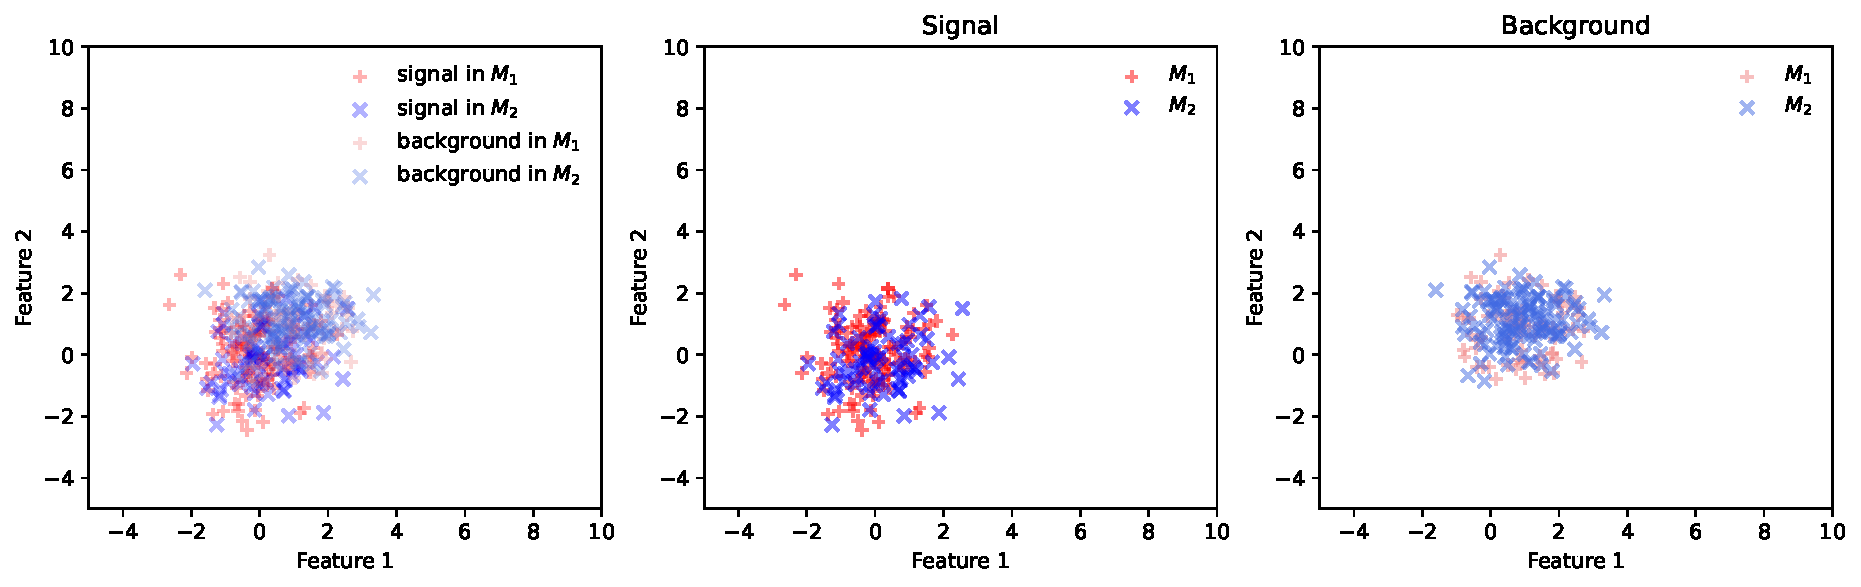
\includegraphics[width=0.97\textwidth]{bootstrapping_training_data_original.pdf}
        \caption{The signal and background samples distributions. The signal and background events are sampled from different two-dimensional normal distributions. They are randomly assigned to the mixed datasets $M_1$ or $M_2$.}
        \label{fig:bootstrapping_signal_background_distribution_origin}
    \end{figure}
    \begin{figure}[htpb]
        \centering
        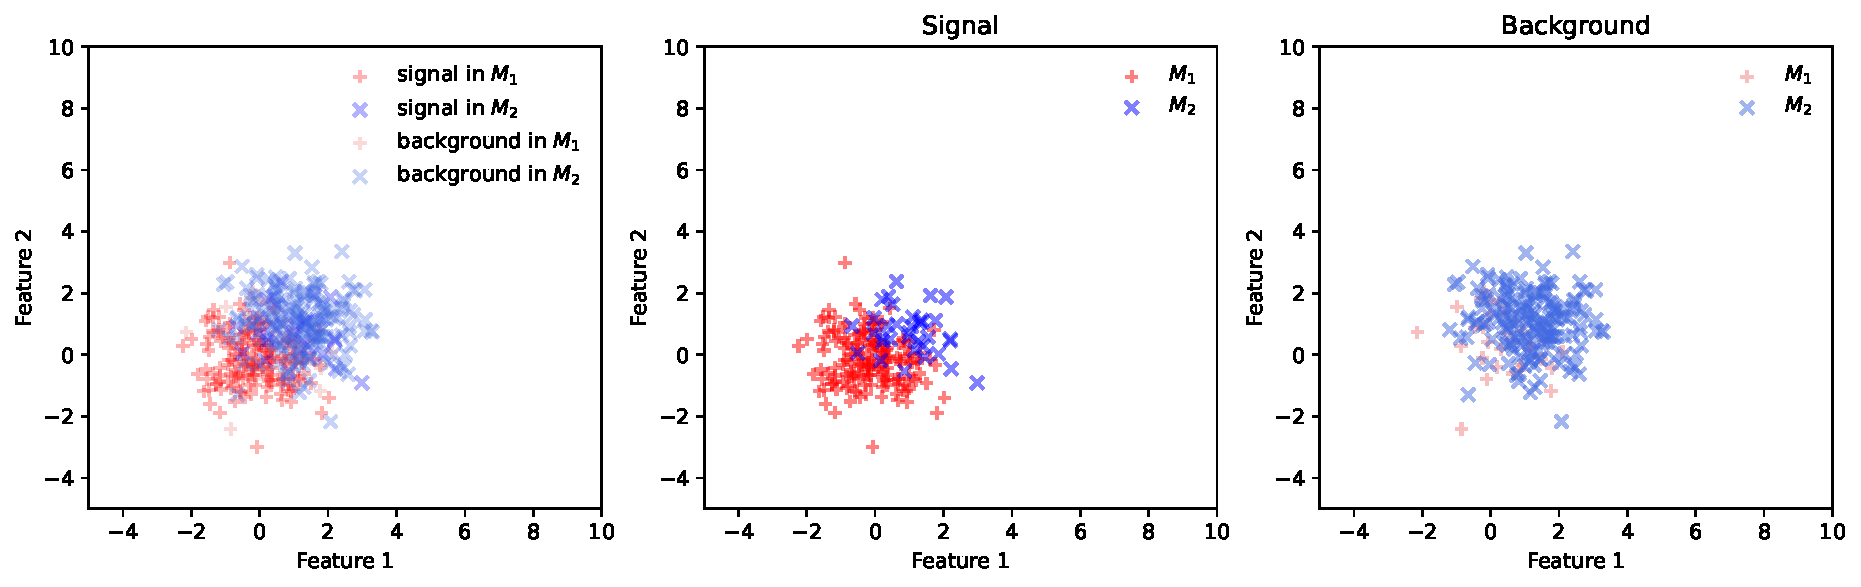
\includegraphics[width=0.97\textwidth]{bootstrapping_training_data_iteration_1.pdf}
        \caption{The signal and background samples distributions. The signal and background events are sampled from different two-dimensional normal distributions. The trained classifier assigns them to the $M_1$ or $M_2$.}
        \label{fig:bootstrapping_signal_background_distribution_iteration_1}
    \end{figure}
% section bootstrapping (end)
\section{Multi-class CWoLa}% (fold)
\label{sec:multi_class_cwola}
    The original CWoLa is only applied to the binary classification tasks. We want to extend the traditional CWoLa to more than two classes.

    \subsection{Dataset and model setup}% (fold)
    \label{sub:dataset_and_model_setup}
        We consider three pure samples, denoted by $A, B$, and $C$. The mixed datasets are denoted by $M_1, M_2$, and $M_3$. The training dataset is sampled from 5-dimensional normal distributions. The number of events in each mixed dataset is 10,000. The testing dataset consists of 1,000 pure samples for each class.

        The neural network consists of two dense layers with eight hidden nodes. The loss function is categorical cross-entropy. To prevent over-training, we utilize the early stopping technique with a patience of 10. The output is a 3-dimensional vector, and each component can be interpreted as the probability belonging to each type.
    % subsection dataset_and_model_setup (end)
    \subsection{Dominated case}% (fold)
    \label{sub:dominated_case}
        To simplify the problem, we start by considering a case where each pure class dominates different mixed samples. This would help us understand the behavior of the multi-class classifier before going to more complex scenarios.

        Table~\ref{tab:type_fraction_dominated_1} lists the fractions of pure samples in mixed datasets. Each mixed dataset is dominated by one pure sample type. Figure~\ref{fig:pure_sample_distribution_dominated_1} illustrates the distributions of the pure classes within these datasets.
        \begin{table}[htpb]
            \centering
            \caption{Fractions of pure samples in mixed datasets.}
            \label{tab:type_fraction_dominated_1}
            \begin{tabular}{c|ccc}
                Dataset & $A$  & $B$  & $C$  \\ \hline
                $M_1$   & 0.70 & 0.20 & 0.10 \\
                $M_2$   & 0.10 & 0.70 & 0.20 \\
                $M_3$   & 0.20 & 0.10 & 0.70
            \end{tabular}
        \end{table}
        \begin{figure}[htpb]
            \centering
            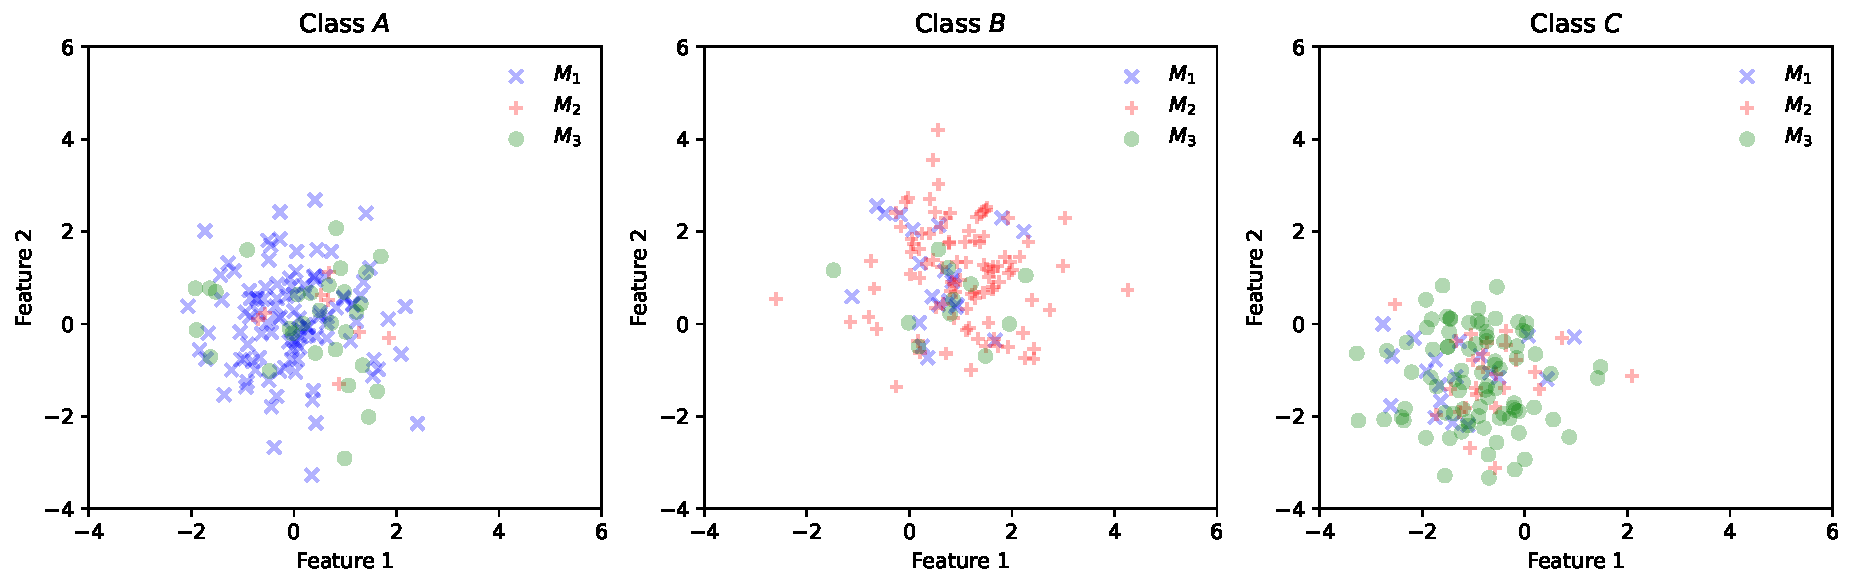
\includegraphics[width=0.97\textwidth]{multi-class_training_data-dominated_1.pdf}
            \caption{Distributions of pure samples in the mixed datasets. The classes $A, B$, and $C$ are sampled from the normal distribution with mean values $0, 1, -1$, respectively.}
            \label{fig:pure_sample_distribution_dominated_1}
        \end{figure}

        If the output vector suggests that the first type has the highest probability for dominated cases, it can be directly interpreted as belonging to the class $A$. The same logic applies to classes $B$ and $C$.  

        The event scores are the components of the output vector. Since the sum of event scores is always 1, we use the ternary plots to represent the event score distributions. In these plots, the coordinate of a point should be read following the direction of the ticks on each axis. 

        Figure~\ref{fig:event_score_distribution_dominated_1} shows the scatter plots of output vectors. The event score distributions are well-separated for each class, indicating successful training. The connections from regions 2 to 1 to 3, due to the mean value of class $B, A$, and $C$, are $1, 0$, and $-1$, respectively.  
        \begin{figure}[htpb]
            \centering
            \subfloat[Training data]{
                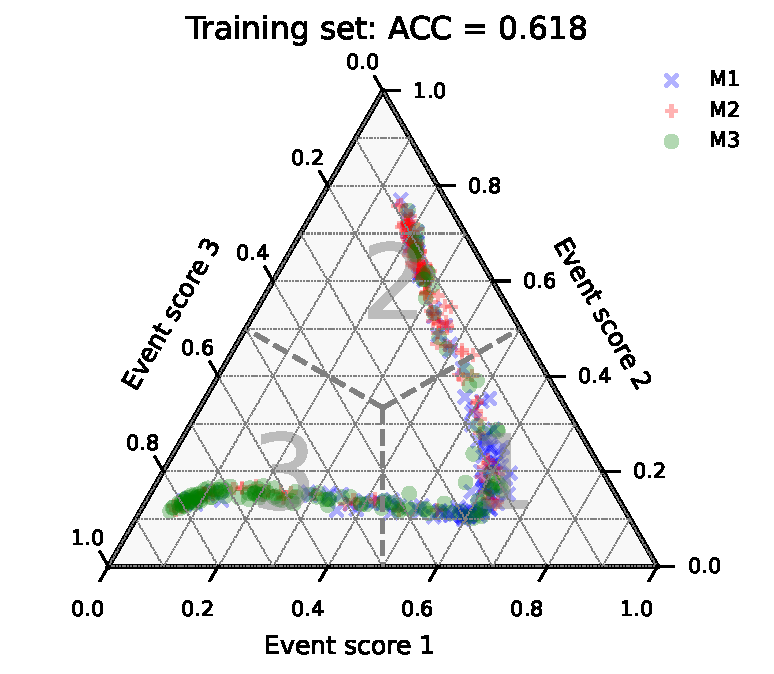
\includegraphics[width=0.47\textwidth]{multi-class_training_data_score-dominated_1.pdf}
            } 
            \subfloat[Testing data]{
                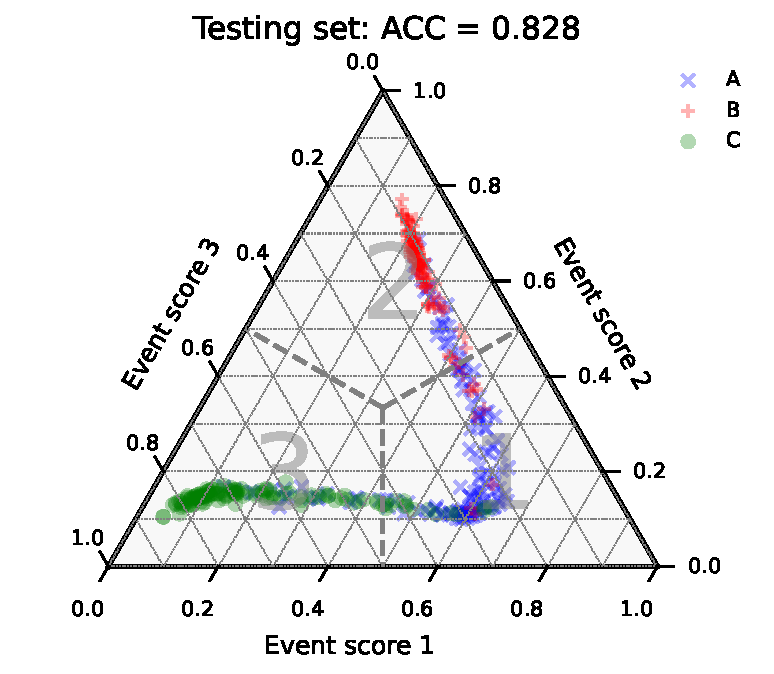
\includegraphics[width=0.47\textwidth]{multi-class_testing_data_score-dominated_1.pdf}
            } 
            \caption{Ternary plots of event score distributions. The grey dashed lines separate the regions corresponding to different classification results. The total accuracy (ACC) and the accuracy for each type are displayed.}
            \label{fig:event_score_distribution_dominated_1}
        \end{figure}  

        Table~\ref{tab:type_fraction_dominated_2} presents another type of the dominated case. Although the pure sample $A$ has the largest fraction in each mixed dataset, the pure class is still dominant in different mixed datasets. Figure~\ref{fig:pure_sample_distribution_dominated_2} illustrates the distributions of the pure classes in these datasets.  
        \begin{table}[htpb]
            \centering
            \caption{Fractions of pure samples in mixed datasets.}
            \label{tab:type_fraction_dominated_2}
            \begin{tabular}{c|ccc}
                Dataset & $A$  & $B$  & $C$  \\ \hline
                $M_1$   & 0.80 & 0.10 & 0.10 \\
                $M_2$   & 0.70 & 0.25 & 0.05 \\
                $M_3$   & 0.60 & 0.20 & 0.20
            \end{tabular}
        \end{table}  

        \begin{figure}[htpb]
            \centering
            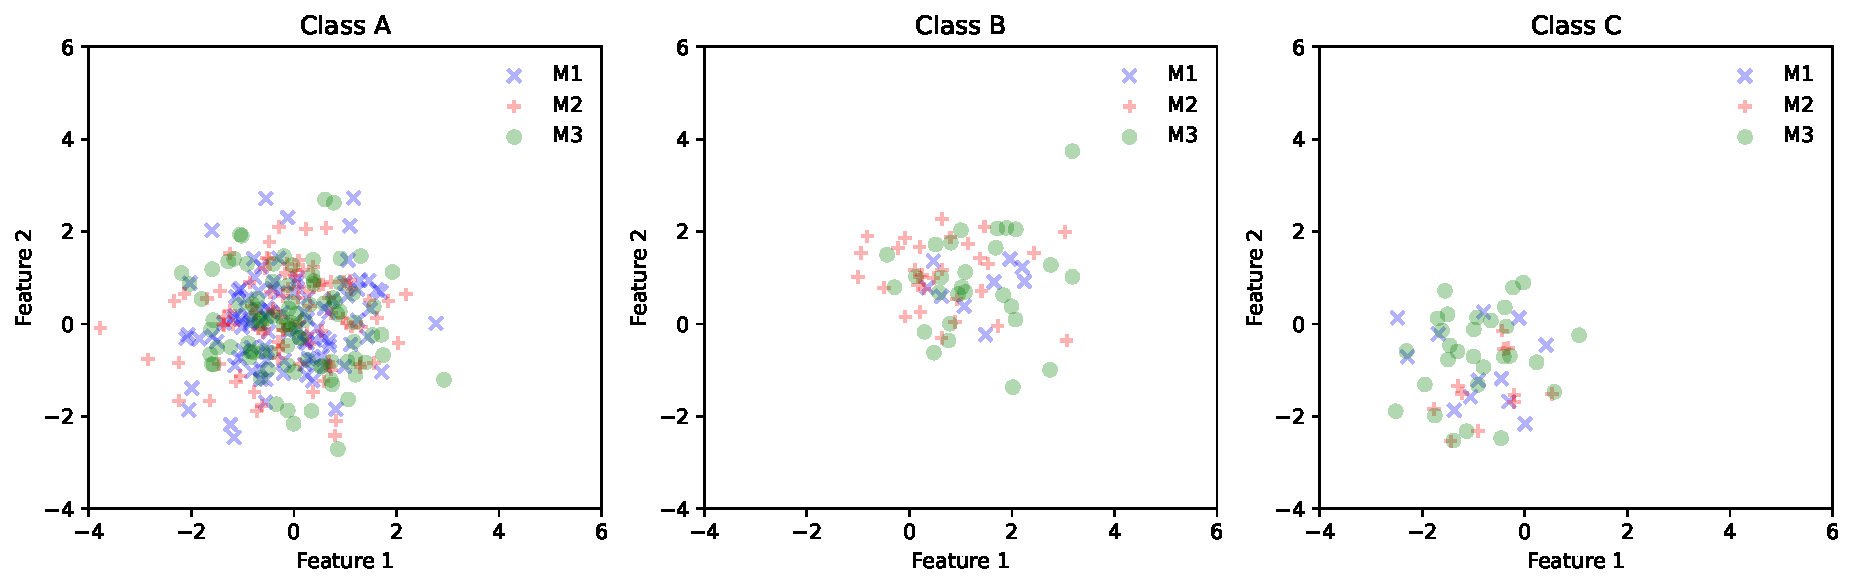
\includegraphics[width=0.97\textwidth]{multi-class_training_data-dominated_2.pdf}
            \caption{Distributions of pure samples in the mixed datasets. The classes $A$, $B$, and $C$ are sampled from normal distributions with mean values $0$, $1$, and $-1$, respectively.}
            \label{fig:pure_sample_distribution_dominated_2}
        \end{figure}  

        Figure~\ref{fig:event_score_distribution_dominated_2} shows scatter plots of output vectors. Although the training accuracy is not good, the testing results demonstrate excellent performance.
        \begin{figure}[htpb]
            \centering
            \subfloat[Training data]{
                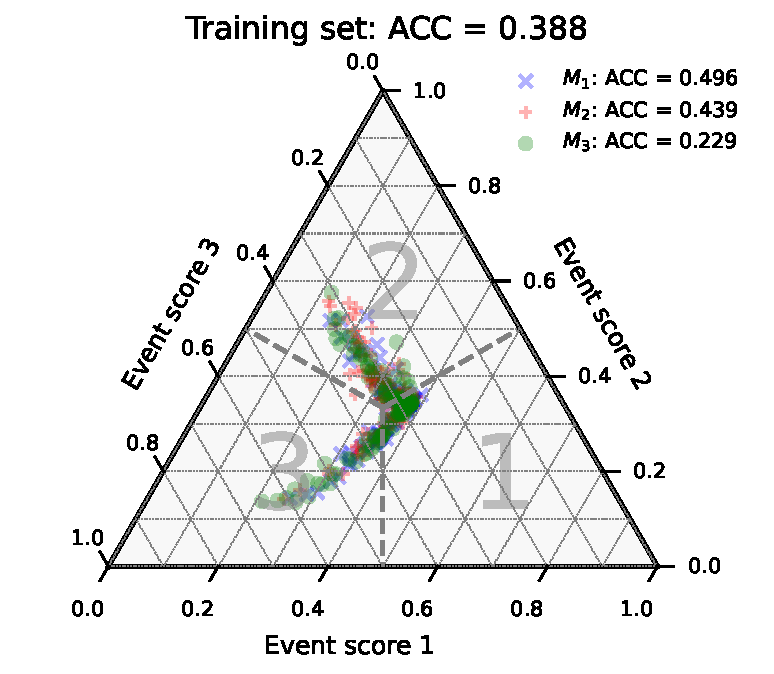
\includegraphics[width=0.47\textwidth]{multi-class_training_data_score-dominated_2.pdf}
            } 
            \subfloat[Testing data]{
                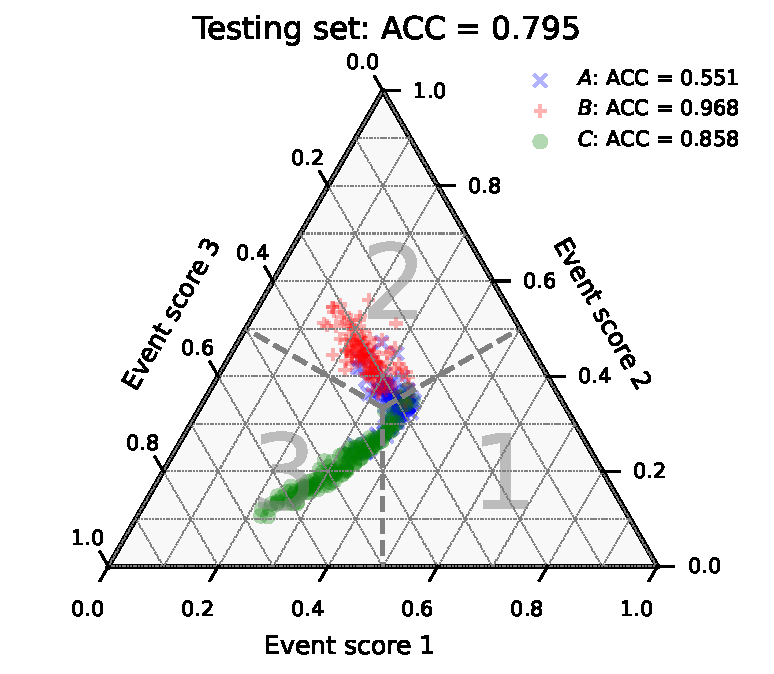
\includegraphics[width=0.47\textwidth]{multi-class_testing_data_score-dominated_2.pdf}
            } 
            \caption{Ternary plots of event score distributions. The grey dashed lines separate the regions corresponding to different classification results. The total accuracy (ACC) and the accuracy for each type are displayed.}
            \label{fig:event_score_distribution_dominated_2}
        \end{figure}

        From these results, we can conclude the ternary CWoLa works for dominated cases.
    % subsection dominated_case (end)
    \subsection{Ambiguous case}% (fold)
    \label{sub:ambiguous_case}
        Table~\ref{tab:type_fraction_ambiguous} lists the fractions of pure samples in mixed datasets. The ambiguous cases mean that the pure sample is not dominant in different mixed datasets. For instance, in table~\ref{tab:type_fraction_ambiguous}, pure samples $B$ and $C$ both dominate in $M_3$. Figure~\ref{fig:pure_sample_distribution_ambiguous} illustrates the distributions of the pure classes within these datasets.
        \begin{table}[htpb]
            \centering
            \caption{Fractions of pure samples in mixed datasets.}
            \label{tab:type_fraction_ambiguous}
            \begin{tabular}{c|ccc}
                Dataset & $A$  & $B$  & $C$  \\ \hline
                $M_1$   & 0.80 & 0.10 & 0.10 \\
                $M_2$   & 0.70 & 0.20 & 0.10 \\
                $M_3$   & 0.60 & 0.25 & 0.15
            \end{tabular}
        \end{table}
        \begin{figure}[htpb]
            \centering
            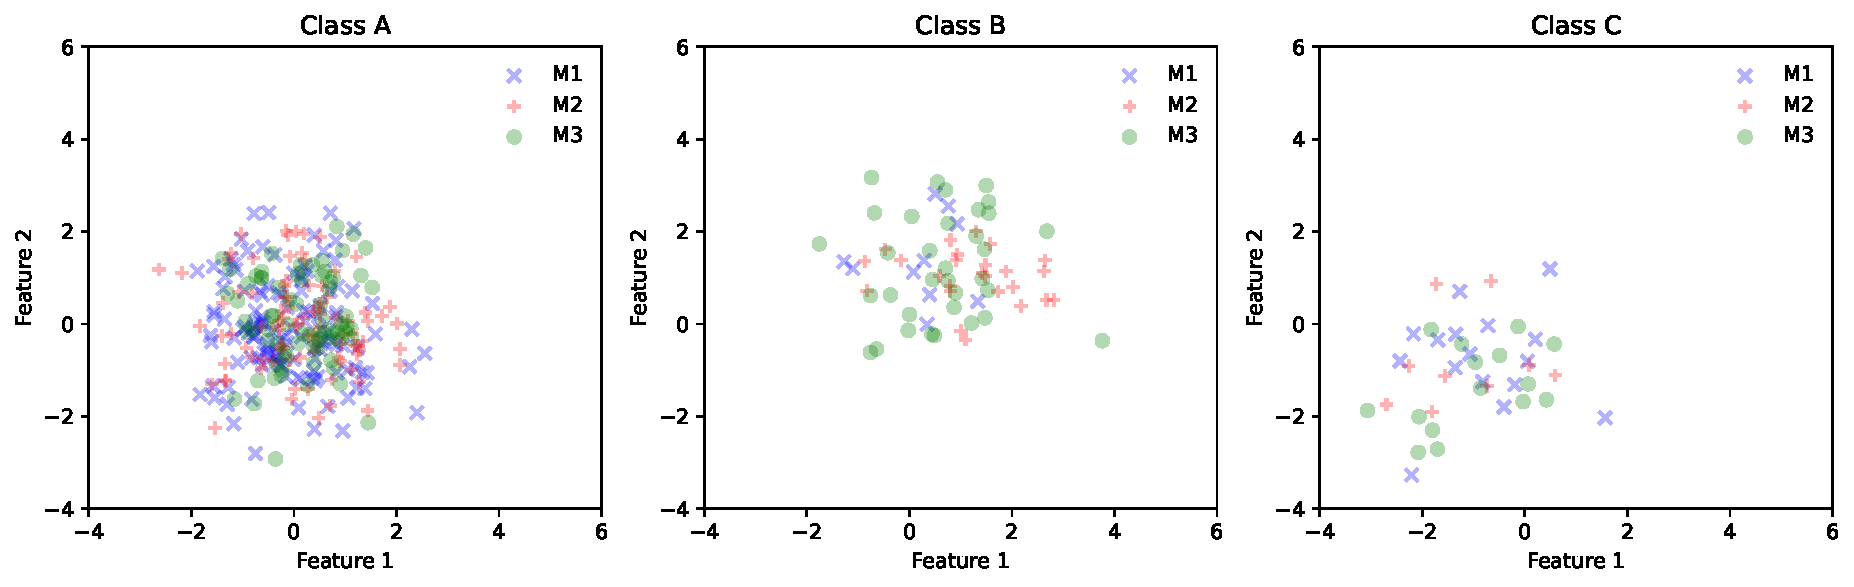
\includegraphics[width=0.97\textwidth]{multi-class_training_data-ambiguous.pdf}
            \caption{Distributions of pure samples in the mixed datasets. The classes $A, B$, and $C$ are sampled from the normal distribution with mean values $0, 1$, and $-1$, respectively.}
            \label{fig:pure_sample_distribution_ambiguous}
        \end{figure}

        For ambiguous cases, we apply the same logic to interpret the output vector as in dominated cases. However, the results could be problematic.

        Figure~\ref{fig:event_score_distribution_ambiguous} shows scatter plots of the output vectors. While the testing accuracy is very low, different types of pure samples exhibit distinct distributions. This suggests that we need another method to interpret the output vector. 

        Note that the accuracy for class $B$ is very low, while the accuracy for class $C$ is significantly higher. This suggests that when the classifier receives an event from either class $B$ or $C$, it tends to assign a high event score of type 3. This behavior is consistent with the fact that the pure samples $B$ and $C$ both are dominated in $M_3$. To improve performance, we need to refine our classification method or better interpret the output vectors.
        \begin{figure}[htpb]
            \centering
            \subfloat[Training data]{
                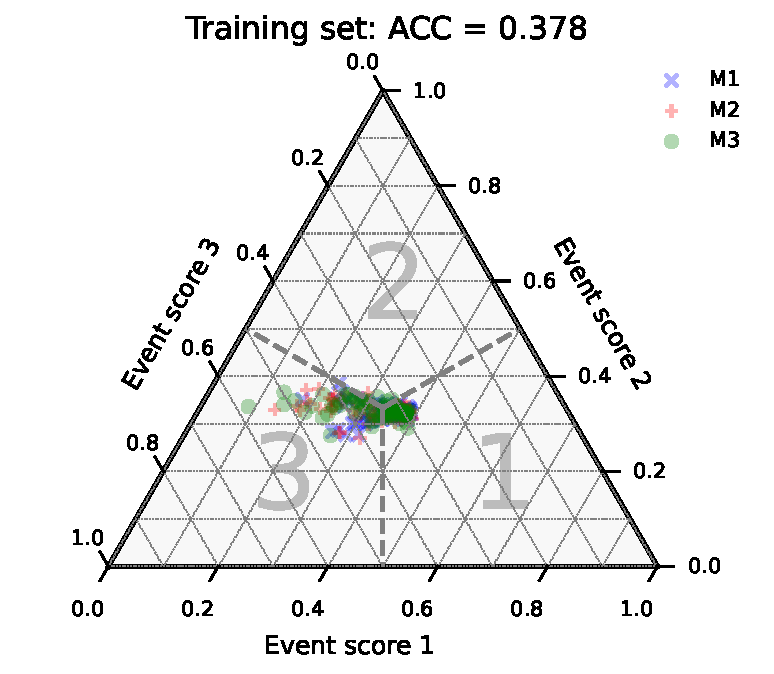
\includegraphics[width=0.47\textwidth]{multi-class_training_data_score-ambiguous.pdf}
            } 
            \subfloat[Testing data]{
                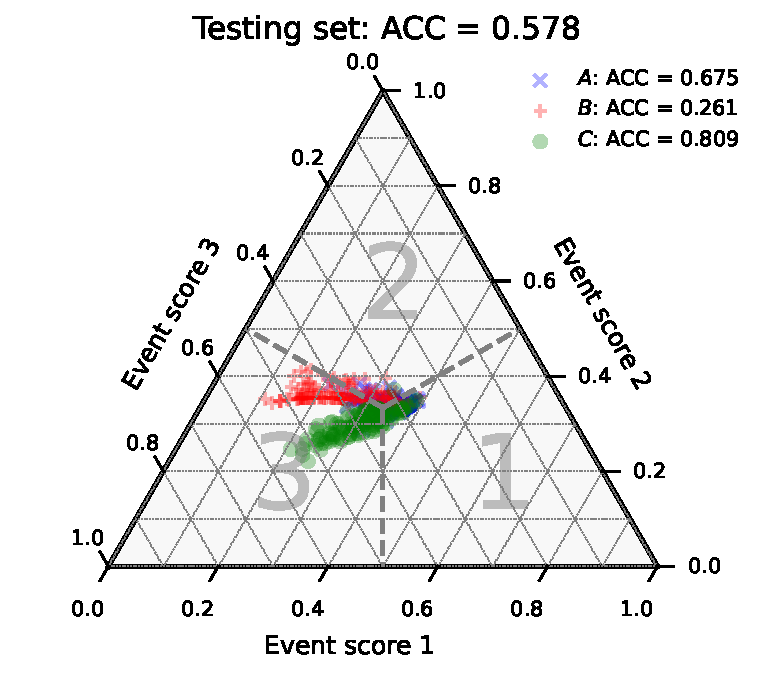
\includegraphics[width=0.47\textwidth]{multi-class_testing_data_score-ambiguous.pdf}
            } 
            \caption{Ternary plots of event score distributions. The grey dashed lines separate the regions corresponding to different classification results. The total accuracy (ACC) and the accuracy for each type are displayed.}
            \label{fig:event_score_distribution_ambiguous}
        \end{figure} 
    % subsection ambiguous_case (end)
% section multi_class_cwola (end)
\end{document}
